\section{Tuesday, May 28}

\todaybox{We will finish our discussion of limits by talking about continuity. We will see that most of the functions we are used to are continuous. However, we will need to be careful when working with branches of multi-valued functions.

This will motivate us to discuss branch cuts, which are a way to find continuous branches of multi-valued functions.}

We've seen a couple of examples of working out limits by hand. In practice, this is a pain. Even in your first year course in calculus, you had tools for working with limits. These same tools, namely the limit laws and continuity, are still applicable in $\C$.

\begin{thmbo}{The Limit Laws}{limlaws}\index{Limit!laws}
Let $f,g:U \rightarrow \C$ and $z_0\in U$. If $\lim_{z\rightarrow z_0} f(z) = A$ and $\lim_{z\rightarrow z_0} g(z) = B$, then:

\begin{itemize}
\item $\lim_{z\rightarrow z_0} \omega = \omega$ for any $\omega \in \C$
\item $\lim_{z\rightarrow z_0} \omega f(z) = \omega A$ for any $\omega \in \C$
\item $\lim_{z\rightarrow z_0} (f+g)(z) = A + B$
\item $\lim_{z\rightarrow z_0} (fg)(z) = AB$
\item If $B\ne 0$, then $\lim_{z\rightarrow z_0} \frac{f}{g}(z) = \frac{A}{B}$.
\end{itemize}
\end{thmbo}

You have a lot of practice using these already. Their application is identical to their use over $\R$. Also, the proofs of these facts are identical to the proofs over $\R$, so we will not reproduce them here.

\subsection{Continuity}

By far the most useful way for finding limits is continuity. If a function is continuous, finding limits for it becomes immediate. So knowing what continuity gives us, and then building up a repetoire of continuous functions, is really important.

\begin{defbo}{Continuity}{continuity}\index{Continuity}
Let $f:U\rightarrow \C$. We say that $f$ is continuous at $z_0 \in U$ if $\lim_{z\rightarrow z_0} f(z) = f(z_0)$. $f$ is called continuous if it is continuous on its domain.
\end{defbo}

So, if we know a function is continuous, then finding limits turns into just evaluating your function at that point.

\begin{ex}{}{} The function $f(z) = e^z$ is continuous.

While this seems like it should be true, we still need to show it. However, if you reproduce our argument for showing that $\lim_{z\rightarrow 0} e^z = 1$, we find:
\begin{align*}\lim_{z\rightarrow x_0 + iy_0} e^z &= \lim_{(x,y) \rightarrow (x_0,y_0)} e^x(\cos(y) + i\sin(y))\\
&= \left(\lim_{x\rightarrow x_0}e^x\right)\left( \lim_{y\rightarrow y_0} \cos(y) + i\sin(y)\right)\\
&= e^{x_0}\left( \lim_{y\rightarrow y_0} \cos(y) + i\lim_{y\rightarrow y_0}\sin(y)\right)\\
&= e^{x_0}(\cos(y_0) + i\sin(y_0))\\
&= e^{z_0}
\end{align*}

\end{ex}

\exercisebox{Prove that $f(z) = z$ is continuous.}

We have a few basic functions, but what about combining them? The limit laws tell us that continuous functions combine very nicely.

\begin{thmbo}{Properties of Continuous Functions}{contprop}\index{Continuity!properties}
Let $f,g$ be functions continuous at $z_0$, and $h$ continuous at $f(z_0)$. Then:

\begin{itemize}
\item Constants are continuous.
\item Constant multiples of $f$ are continuous at $z_0$.
\item Sums, differences, and products of $f$ and $g$ are continuous at $z_0$.
\item If $g(z_0)\ne 0$, then $\frac{f}{g}$ is continuous at $z_0$.
\item $h\circ f$ is continuous at $z_0$.
\end{itemize}
\end{thmbo}

As a result of this, most of the functions we've seen so far are continuous. Constants, polynomials, exponentials, and our trig functions are continuous.

What about logarithms, or the argument?

\begin{ex}{}{} Let $\arg_0(z)$ be the branch of the argument defined by setting $\arg_0(z) \in [-\pi,\pi)$.

Find $\lim_{z\rightarrow -1} \arg_0(z)$.

Since this limit needs to exist and agree regardless of which direction we approach $-1$ from, we're going to approach along two curves: we're going to follow the unit circle to $-1$ from above and from below.

\begin{center}
\begin{tikzpicture}
%\draw [help lines,black!20!white] (-1,-1) grid (4,4);

\draw[thick] (0,-2) -- (0,2);
\draw[thick] (-2,0) -- (2,0);


\draw [red,thick,domain= 100:180, ->, dashed] plot ({cos(\x)}, {sin(\x)});
\draw [blue,thick,domain= 260:180, ->] plot ({cos(\x)}, {sin(\x)});

\end{tikzpicture}
\end{center}


First, let's discuss what happens if we follow the curve $z = e^{i\theta}$ as it approaches $-1$ from above (i.e., as we follow the red, dashed curve.) Notice that since we are in the second quadrant, that $\arg_0(z) \in \left(\frac{\pi}{2},\pi\right]$, and so we see that:
$$\theta \rightarrow \pi^{-}$$

As such, $\lim_{z\rightarrow -1} \arg_0(z) = \lim_{\theta \rightarrow \pi^-} \theta = \pi$.

On the other hand, if we approach $-1$ from below along the blue, solid curve, we see that $\arg_0(z) \in \left(-\pi,\frac{-\pi}{2}\right)$, and so:
$$\theta\rightarrow -\pi^+$$

And so, in a similar way to the previous curve, we find that $\lim_{z\rightarrow -1} \arg_0(z) = -\pi$.

Since the limit approaches two different values, it does not exist. Also, as a consequence, we see that $\arg_0(z)$ is not continuous at $-1$.
\end{ex}

\begin{note} A similar argument will show that $\arg_0$ and $\log_0$ are not continuous on $(-\infty,0]$, but that they are continuous on $\C \setminus (-\infty, 0]$.

This is why we defined $\Arg(z)$ and $\Log(z)$ to have the domain $\C\setminus (-\infty,0]$. We want to work with continuous (actually, differentiable) functions, and so we define these functions on a set where they are continuous.\end{note}

The issue here is that $\arg(z)$ and $\log(z)$ are multivalued functions. As we move around the circle $|z| = 1$:

\begin{center}
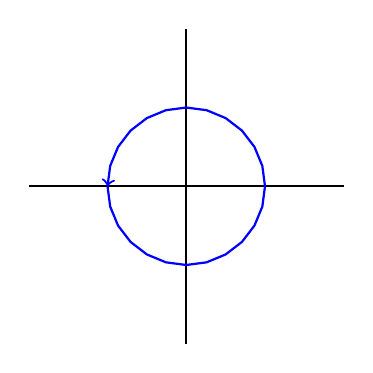
\begin{tikzpicture}
%\draw [help lines,black!20!white] (-1,-1) grid (4,4);

\draw[thick] (0,-2) -- (0,2);
\draw[thick] (-2,0) -- (2,0);

\draw [blue,thick,domain= -180:180, ->] plot ({cos(\x)}, {sin(\x)});

\end{tikzpicture}
\end{center}

\noin the value of $\arg(z)$ increases by $2\pi$, and the value of $\log(z)$ increases by $2\pi i$. The same thing happens with other multivalued functions.

\begin{ex}{}{} What happens to $z^{\frac{1}{2}}$ and $z^{\frac{1}{3}}$ if we travel around the unit circle?

For $z^{\frac{1}{2}}$, we use the formula $\sqrt{r}e^{i\frac{\theta}{2}}$. So, starting at $1$ written as $e^{i0}$, we have $1^{\frac{1}{2}} = 1$. As we move around the circle once (clockwise), we see that $\theta$ moves from $0$ to $2\pi$, and so $z^{\frac{1}{2}}$ moves from $e^{i0} = 1$ to $e^{i\pi} = -1$. Pictorially:

\begin{center}
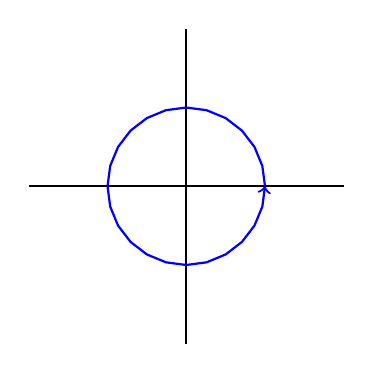
\begin{tikzpicture}[baseline=(current bounding box.center)]
%\draw [help lines,black!20!white] (-1,-1) grid (4,4);

\draw[thick] (0,-2) -- (0,2);
\draw[thick] (-2,0) -- (2,0);

\draw [blue,thick,domain= 0:360, ->] plot ({cos(\x)}, {sin(\x)});

\end{tikzpicture}
\qquad$\longrightarrow$\qquad
\begin{tikzpicture}[baseline=(current bounding box.center)]
%\draw [help lines,black!20!white] (-1,-1) grid (4,4);

\draw[thick] (0,-2) -- (0,2);
\draw[thick] (-2,0) -- (2,0);

\draw [blue,thick,domain= 0:180, ->] plot ({cos(\x)}, {sin(\x)});

\end{tikzpicture}
\end{center}

And to get back to $1$, we need to go around the unit circle twice!

A similar line of reasoning applies to the multi-valued function $z^{\frac{1}{3}}$. In this case, the picture looks like:

\begin{center}
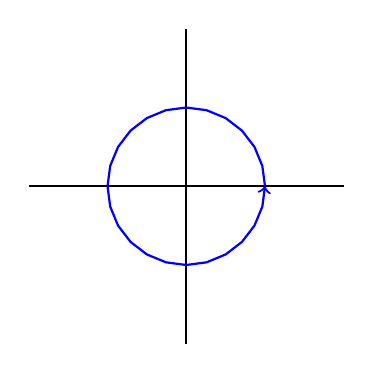
\begin{tikzpicture}[baseline=(current bounding box.center)]
%\draw [help lines,black!20!white] (-1,-1) grid (4,4);

\draw[thick] (0,-2) -- (0,2);
\draw[thick] (-2,0) -- (2,0);

\draw [blue,thick,domain= 0:360, ->] plot ({cos(\x)}, {sin(\x)});

\end{tikzpicture}
\qquad$\longrightarrow$\qquad
\begin{tikzpicture}[baseline=(current bounding box.center)]
%\draw [help lines,black!20!white] (-1,-1) grid (4,4);

\draw[thick] (0,-2) -- (0,2);
\draw[thick] (-2,0) -- (2,0);

\draw [blue,thick,domain= 0:120, ->] plot ({cos(\x)}, {sin(\x)});

\end{tikzpicture}
\end{center}

In this case, as we travel the unit circle once, $z^{\frac{1}{3}}$ goes from $1$ to $\omega_1 = e^{i\frac{2\pi}{3}}$, which is another cube root of unity.
\end{ex}


So what's the solution to this problem? We want to work with continuous functions, if we're going to talk about differentiation. We've seen an example already: for $\log(z)$, we restricted the domain to $\C\setminus (-\infty,0]$, and we were able to find a branch on that domain which is continuous.

This leads us to a more general phenomenon.

\subsection{Branch Cuts}

The idea behind branch cuts is to find a way to take discontinuous branches of a multi-valued function, and to remove a portion of the domain to get a continuous function.

\begin{defbo}{Branch Cuts}{branchcut}\index{Branch!cut} Let $f(z)$ be a branch of a multi-valued function. A branch cut is a curve in $\C$ along which $f(z)$ is discontinuous.\end{defbo}

It is called a branch {\bf cut} because we cut (i.e. remove) the branch cut from the domain to get a continuous function.

\begin{ex}{}{} Let $\log_0(z)$ be the branch of the logarithm given by $\arg(z) \in [-\pi,\pi)$. As we saw earlier, $\log_0(z)$ is discontinuous along $(-\infty,0]$, and so this is a branch cut. Removing $(-\infty,0]$ from the domain of $\log_0(z)$ results in the function $\Log(z)$, which is continuous on its domain.
\end{ex}

All of the multi-valued functions we have seen so far are defined in terms of $\log(z)$ or $\arg(z)$. As such, we can get branch cuts for them by taking branch cuts for $\log(z)$ or $\arg(z)$. Let's start by talking about how to do that.

Consider the branch $\log_0(z)$ of $\log(z)$ given by $\arg(z) \in (\theta, \theta + 2\pi)$ for some $\theta \in \R$. This function is continuous on its domain, in the same way that $\Log(z)$ is continuous on $\C\setminus(-\infty,0]$. We have removed the ray $\{re^{i\theta}|r\ge 0\}$, pictured below:

\begin{center}
\begin{tikzpicture}[baseline=(current bounding box.center)]
%\draw [help lines,black!20!white] (-1,-1) grid (4,4);

\draw[thick] (0,-2) -- (0,2);
\draw[thick] (-2,0) -- (2,0);

\draw[semithick, ->] (0,0) -- (1.3,1.9);

\end{tikzpicture}
\end{center}

\noin By taking this branch cut, we have found a continuous branch. In practice, these are the only types of branch cuts we will consider.

Now that we have a standard way of taking branch cuts for $\log(z)$ or $\arg(z)$, how do these choices affect other multivalued functions?

\begin{ex}{}{} Consider $f(z) = (iz + 1)^{\frac{1}{2}}$, where we are working with the principal branch. What is the branch cut of this function?

Since we are asking about a branch cut, this should serve as a huge clue that this function involves $\log(z)$ somehow. Recall that $(iz+1)^{\frac{1}{2}} = e^{\frac{1}{2}\Log(iz+1)}$.

Now, our branch cut on $\Log(z)$ is to remove $(-\infty,0]$ from the domain. So the corresponding branch cut for $f(z)$ is to remove where $iz + 1 \in (-\infty,0]$.

Suppose $iz + 1 \in (-\infty,0]$. Then $iz \in (-\infty,-1]$. As such, $z\in \left\{\frac{r}{i}|r \le -1\right\} = \{si|s\ge 1\}$. As such, our branch cut is the positive imaginary axis above $1$.
\end{ex}

\subsection{Infinite Limits and Limits at Infinity}

The last thing to consider is infinite limits and limits at infinity. The key concept here is that in $\C$, there is only one $\infty$. No matter which direction you go out in, left or right, up or down, you get to the same infinity. This is tied to the notion of the Riemann sphere, and of Riemann surfaces, which are a geometric abstraction that makes a lot of complex analysis very nice. We won't be talking in this context in this course. I am pointing these out in case you are interested in further reading.

So, how do we define infinite limits? Well, $f(z)$ should be going to $\infty$. But what way? Well, since all directions give the same $\infty$, any way!

\begin{defbo}{Infinite Limits}{inflim}\index{Limit!infinite}
Let $f:U\rightarrow \C$ and $z_0\in \C$, such that $\{z\in \C| 0 <|z-z_0|< r\} \subset U$ for some $r>0$. Then we say that $\lim_{z\rightarrow z_0} f(z) = \infty$ if:

$$\forall N > 0, \exists \delta > 0 \text{ such that } 0 < |z-z_0| < \delta \implies |f(z)| > N$$
\end{defbo}

In laymans terms, this means that $|f(z)|$ gets arbitrarily large as we get close to $z_0$.

\begin{ex}{}{} Is $\lim_{z\rightarrow 0} e^{\frac{1}{z}}$ infinite or not?

Well, for example, if we consider $z\rightarrow 0$ along the positive real axis, we find that $e^{\frac{1}{x}}$ does go to infinity. After all, $\lim_{x\rightarrow 0^+}\frac{1}{x}=\infty$.

However, consider what occurs as $z\rightarrow 0$ along the positive imaginary axis. We have that $e^{\frac{1}{z}} = e^{\frac{1}{ri}} = e^{\frac{-i}{r}}$. And so $|e^{\frac{1}{z}}| = 1$. As such, if we approach from this direction, $e^{\frac{1}{z}}$ does not approach $\infty$.

So this limit is not infinite.
\end{ex}

What about limits at infinity?

\begin{defbo}{Limits at Infinity}{limatinf}\index{Limit!at infinity}
Let $f:U\rightarrow \C$ such that $\{z\in \C| |z| > r\} \subset U$ for some $r > 0$. Then we say that $\lim_{z\rightarrow \infty} f(z) = L$ if:

$$\forall \varepsilon > 0, \exists M > 0 \text{ such that } |z| > M \implies |f(z) - L| < \varepsilon$$
\end{defbo}

Or, in laymans terms, as $|z|$ gets arbitrarily large, $f(z)$ gets arbitrarily close to $L$.

\begin{ex}{}{} Show that $\lim_{z\rightarrow \infty} z = \infty$.

So, we haven't defined this, but hopefully seeing the two separate definitions allows us to synthesize the correct definition of an infinite limit at infinity.

In this case, we want that as $|z|$ gets arbitrarily large, that $|f(z)| = |z|$ gets arbitrarily large, which is obviously the case.
\end{ex}